\subsection{Differential Evolution Method}
%The method in chapter \ref{sec:lossFunc} requires the objective function must be differentiable to evaluate the effect of perturbation on the final prediction.
Besides gradient descent, differential evolution (DE) or genetic method is another algorithm for solving optimization problems \cite{onePixel}. DE is a population-based optimization algorithm, its work principle could be briefly summarized as ``natural selection'' or ``survival of the fittest''. As the name implies, DE generates a new candidate set (children) from the current set (parent), and only keeps the candidates with the highest criteria (e.g. fitness value, diversity\dots) for the next iteration.

The prominent advantage of DE lies in three aspects: it is independent of whether the model is differentiable, and does not require internal gradients, this is the very case with a ``black-box'' model. Secondly, it is applicable for any sort of input data (continuous/categorical tabular data or image data). And finally, DE suffers less from local minima than gradient descent, partially due to the diversity in the candidate set.

The main steps of the genetic method are listed as follow \cite{certifai}:
\begin{enumerate}
  \item randomly generate points that belong to a CF class
  \item choose candidates with largest fitness value, where fitness equals the inverted distance to the original data input, i.e. $fitness=\frac{1}{d(\textbf{x,c})}$
  \item mutate the candidates by arbitrarily changing their values
  \item randomly exchange some feature between candidates
\end{enumerate}
The steps are repeated until the maximum iteration is reached, and one single candidate with the best fitness is selected.

Similarly, another DE application of searching CF examples for image data is given by \citeauthor{onePixel} \cite{onePixel}. The result is impressive, see \autoref{fig:onepixel}, because the CF has only one pixel changed compared to the original data. The evaluation formula as following:
\begin{equation}\label{eq:onepixel}
  \begin{split}
     &\max_{\mathbf c^\star} f_{i_c}(\mathbf{c})\\
     &subject\ to\ ||\mathbf{x-c}||_0=1
  \end{split}
\end{equation}
The formula maximizes the prediction possibility of the target CF class $i_c$, while constraining the CF to be only one pixel different from the input. The 0-norm measures the number of non-zero elements, ensuring the sparsity.
\begin{figure}
  \centering
  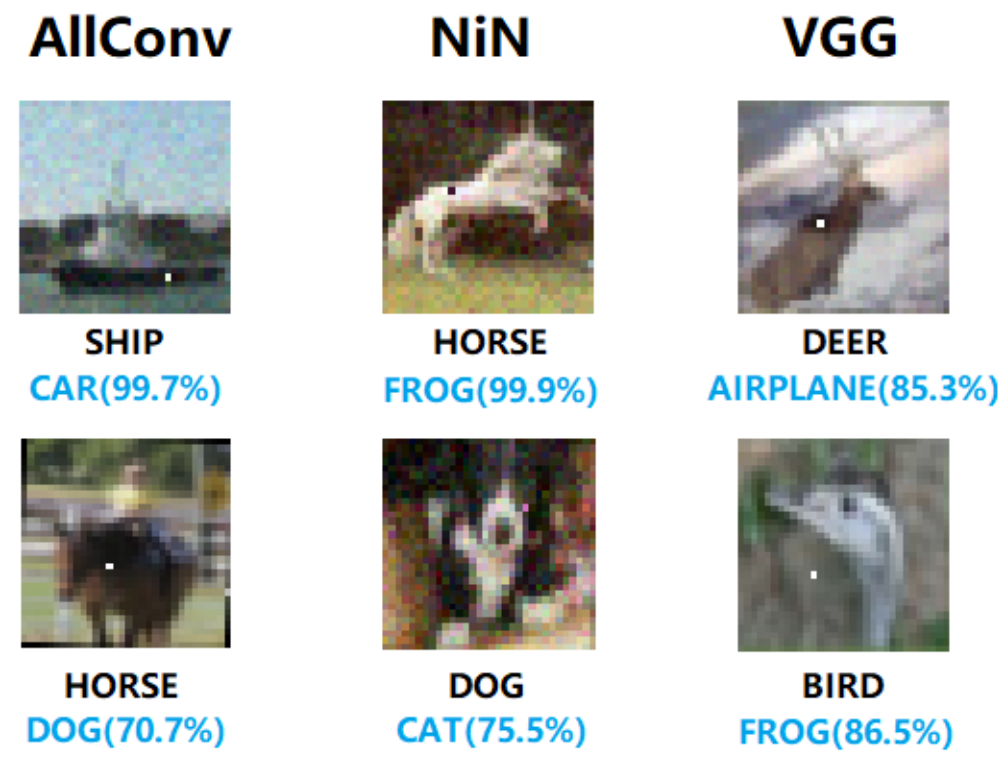
\includegraphics[width=0.5\textwidth]{onepixel.PNG}
  \caption{one-pixel different CFs on CIFAR-10 dataset, a dataset that consists of $32\times32$ large images in 10 classes.
  The first row beneath each image is the original class, and the second row is the CF class. All three networks give out high confidence for the CF examples. Credit: \cite{onePixel}
  }
  \label{fig:onepixel}
\end{figure}

